\documentclass{article}
\usepackage[spanish]{babel}
\decimalpoint
\usepackage[utf8]{inputenc}
\usepackage{listings}
\usepackage{graphicx}
\usepackage{amsmath}

\usepackage{subcaption}

\setlength{\parskip}{0.5em}

\title{Reporte de Programa y Usos}
\author{Rodrigo Moreno}
\date{\today}

\begin{document}
\maketitle

Escribí un código que descompone el problema en varios objetos. Primero que nada, se debe definir un objeto que contiene los parámetros del sistema \texttt{i\_max}, \texttt{u\_max}, \texttt{gamma} y \texttt{beta}. Este objeto es de una clase llamada \texttt{SIR}. Se comienza el código con los siguientes comandos:
\begin{lstlisting}[basicstyle = \ttfamily]%, language = Python]
from sir import *

imax = 0.1
umax = 0.5
gamma = 0.2
beta = 0.5

A = SIR()
A.set_params(imax, umax, gamma, beta)
A.find_tau()
A.find_psi()
A.find_theta()
A.find_rho()
\end{lstlisting}
La clase \texttt{SIR} tiene diferentes métodos. Entre ellos, los importantes son \texttt{SIR.find\_tau()}, \texttt{SIR.find\_psi()}, \texttt{SIR.find\_theta()} y \texttt{SIR.find\_rho()}. Estos métodos permiten encontrar cuatro curvas distintas (fig. \ref{fig:regiones}), que a su vez permiten generar las trayectorias desde un punto inicial. Cada una de estas curvas es de una clase \texttt{CurveSegment()}, de la cual se va a comentar más adelante, accesible como atributos de \texttt{A}: \texttt{A.tau}, \texttt{A.phi}, \texttt{A.theta} y \texttt{A.rho}. La curva \texttt{A.tau} es aquella con máximo en $[\tfrac{\gamma}{\beta}, I_{max}]$, se calcula con $u = 0$, y es la frontera para la zona <<segura>>. \texttt{A.phi} tiene máximo en $[\tfrac{\gamma}{(1-u_{max})\beta}, I_{max}]$ y se genera con $u = u_{max}$. \texttt{A.theta} inicia donde \texttt{A.tau} cruza 0, es con $u = u_{max}$ y tiene máximo en $\frac{\gamma}{(1-u_{max})\beta}$. Finalmente, \texttt{A.rho} es la curva que pasa por $\frac{\gamma}{(1-u_{max})\beta}$ con $u = 0$. De ahora en adelante, $\bar{S} = \tfrac{\gamma}{\beta}$ y $S^* = \tfrac{\gamma}{(1 - u_{max})\beta}$.

\begin{figure}
\centering
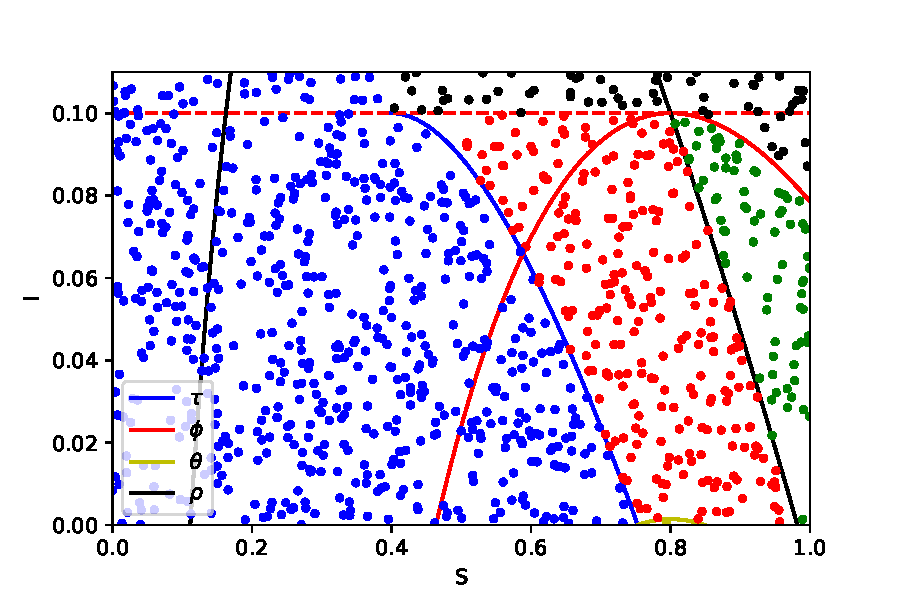
\includegraphics[width = \textwidth]{regions.pdf}
\caption{Curvas y regiones del sistema, generadas a partir de los parámetros mostrados arriba en el código. Los puntos azules, rojos, verdes, amarillos y negros pertenecen a las regiones 1, 2, 3, 4 y 5, respectivamente.}
\label{fig:regiones}
\end{figure}

La siguiente parte del código implica la generación de una condición inicial:
\begin{lstlisting}[basicstyle = \ttfamily]
s0 = 0.6
i0 = 0.08
P = Point(s0, i0, A)
P.find_region()
\end{lstlisting}
La inicialización de un punto se hace con las coordenadas de origen \texttt{s0} e \texttt{i0}, y el sistema al que pertenece, en este caso \texttt{A}. El punto va a heredar ciertos atributos del sistema al que pertenece. El método \texttt{P.find\_region()} crea un atributo de la clase que determina en qué región del sistema se encuentra con respecto a sus curvas (fig. \ref{fig:regiones}). Dependiendo de la región en la que se encuentre el punto, cambia el método para generar las trayectorias. A grandes razgos:
\begin{enumerate}
\item No se requiere generar una trayectoria, ya que ya está en la región deseada.

\item Se genera una trayectoria principal, compuesta de dos segmentos. El primer segmento con $u = 0$ hasta llegar a $I_{max}$, y el segundo un \texttt{LineSegment} por la curva singular hasta llegar a $\bar{S}$. El resto de las trayectorias se genera haciendo \texttt{CurveSegment} con $u = u_{max}$ desde cualquier punto de la trayectoria principal hasta algún punto en \texttt{A.tau}.

\item Se genera una trayectoria principal compuesta por tres segmentos. El primero es un \texttt{CurveSegment} con $u = 0$ desde el punto inicial hasta \texttt{A.phi}. El segundo es la curva siguiendo a \texttt{A.phi} hasta llegar a $S^*$. El tercero es un \texttt{LineSegment} por la curva singular hasta $\bar{S}$. El resto de las trayectorias se genera haciendo \texttt{CurveSegment} con $u = u_{max}$ desde diferentes puntos del primer o tercer segmento, hasta llegar a \texttt{A.tau}.

\item Los puntos en esta región deben primero salir de ella con $u = 0$. La salida puede ser a cualquiera de las regiones 2, 3 o 5, por lo cual la construcción de las trayectorias se hace dependiendo de a cuál salga.

\item No se generan trayectorias porque ninguna de ellas cumple con el criterio de no sobrepasar $I_{max}$. Por ahora, éste es un método vacío, pero se puede adaptar a las necesidades que puedan surgir más adelante.
\end{enumerate}

Finalmente, las trayectorias y los tiempos de cada una se pueden generar utilizando
\begin{lstlisting}[basicstyle = \ttfamily]
T = TrajectoryCreator(P)
trajectories = T.get_trajectories()

for trajectory in trajectories:
	trajectory.get_time()
times = [trajectory.time for trajectory in trajectories]
ends = [trajectory.s[-1] for trajectory in trajectories]
\end{lstlisting}
El objeto \texttt{TrajectoryCreator} toma como argumento un objeto de clase \texttt{Point}. El método \texttt{TrajectoryCreator.get\_trajectories()} genera una lista de objetos \texttt{Trajectory} compuestos de segmentos \texttt{CurveSegment} o \texttt{LineSegment}, cada uno con métodos para calcular sus tiempos dependiendo de la clase. La clase \texttt{Trajectory} también cuenta con un método para calcular su tiempo, que calcula y suma los tiempos de cada uno de sus segmentos. Una muestra de las trayectorias generadas para el punto inicial mostrado arriba se presenta en la figura \ref{fig:trajectories}. Los arreglos \texttt{times} y \texttt{ends} contienen los tiempos de cada trayectoria, y la coordenada en $S$ de cada punto de intersección con \texttt{A.tau}. Estos se pueden graficar para ver las tendencias (fig. \ref{fig:times}).

\begin{figure}
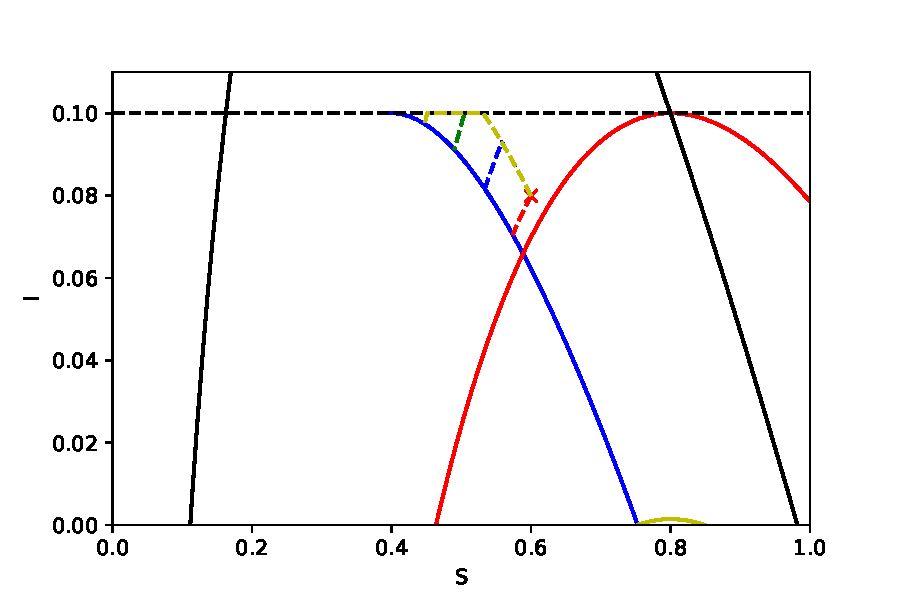
\includegraphics[width = \textwidth]{trajectories.pdf}
\caption{Muestra de trayectorias del punto \texttt{P}.}
\label{fig:trajectories}
\end{figure}

\begin{figure}
\centering
\begin{subfigure}{0.5\textwidth}
	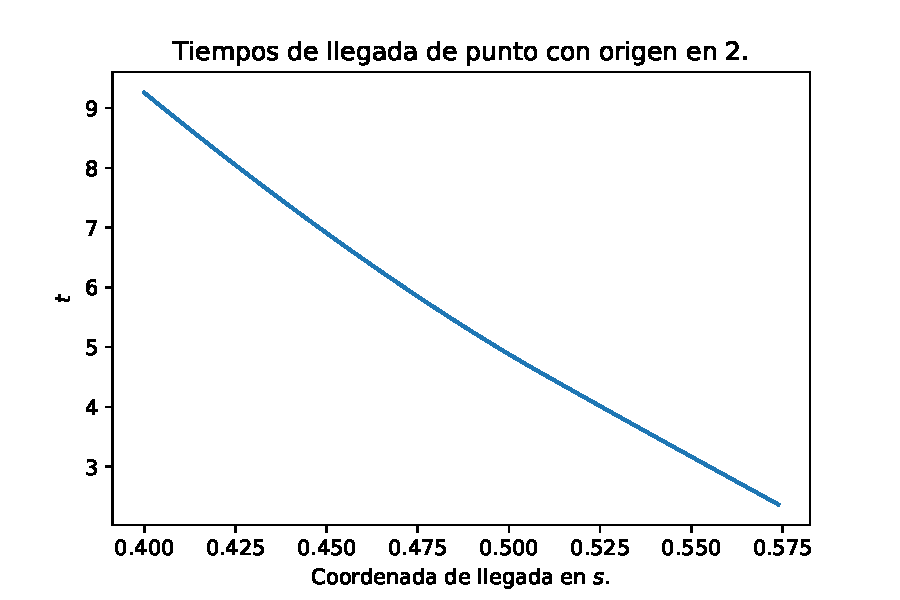
\includegraphics[width = \textwidth]{tiempos_2.pdf}
	\caption{}
	\label{subfig:2}
\end{subfigure}%%%
\begin{subfigure}{0.5\textwidth}
	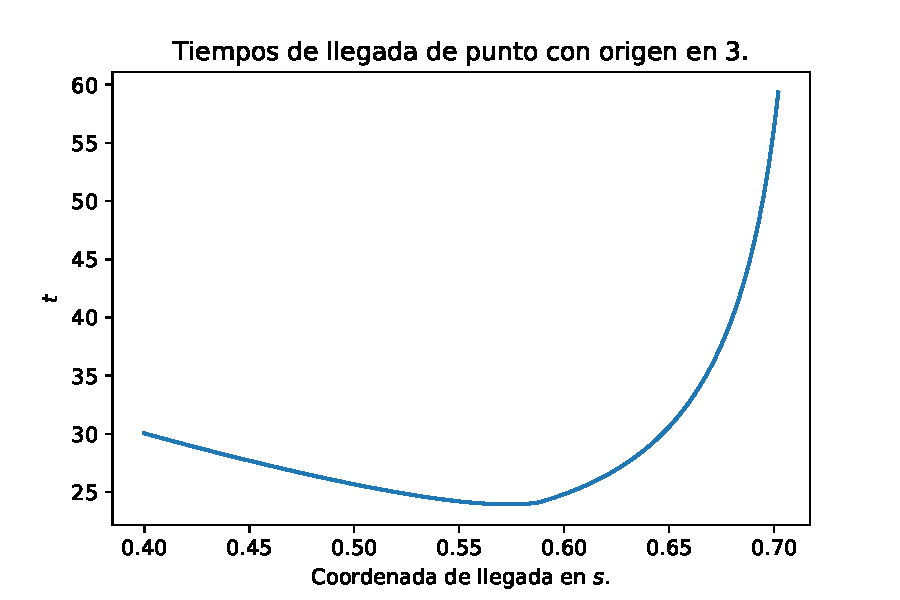
\includegraphics[width = \textwidth]{tiempos_3.pdf}
	\caption{}
	\label{subfig:3}
\end{subfigure}

\begin{subfigure}{0.5\textwidth}
	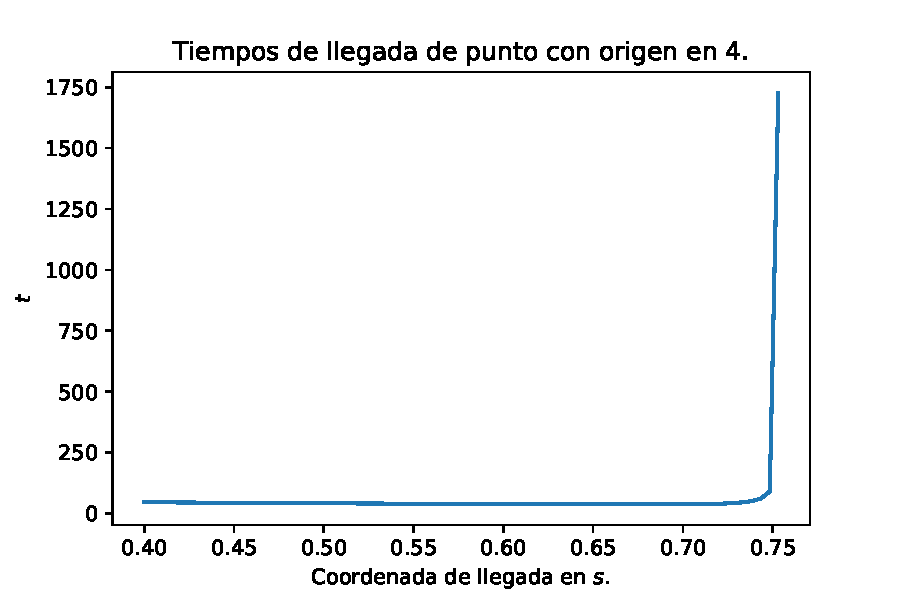
\includegraphics[width = \textwidth]{tiempos_4.pdf}
	\caption{}
	\label{subfig:4}
\end{subfigure}
\caption{Coordenada contra tiempo de llegada de trayectorias iniciadas en las regiones 2 (\ref{subfig:2}), 3 (\ref{subfig:3}) y 4 (\ref{subfig:4}). Los puntos iniciales son los mostrados arriba (\ref{subfig:2}), $[1 - 1e^{-2}, 1e^{-2}]$ (\ref{subfig:3}) y $[0.8, 1e^{-4}]$ (\ref{subfig:4}).}
\label{fig:times}
\end{figure}

Los tiempos de integración se corroboraron haciendo simulaciones del sistema dinámico. Se generó un objeto \texttt{CurveSegment} con condiciones iniciales en $[0.6, 0.08]$ y $u = u_{max}$ (fig. \ref{fig:integral}, puntos rojos), y se calculó el tiempo $t_f$ asociado a él. Por otro lado, se hizo una simulación del sistema con las mismas condiciones (mismos valores de parámetros y condiciones iniciales), con $t_0 = 0$ y tiempo máximo $t_f$. La trayectoria simulada del sistema se muestra en la figura \ref{fig:integral} con cruces rojas. Ya que ambas curvas son iguales, se puede concluir que el resultado obtenido por la integración es correcto. De lo contrario, la curva obtenida por la simulación del sistema sería de una extensión diferente.

\begin{figure}
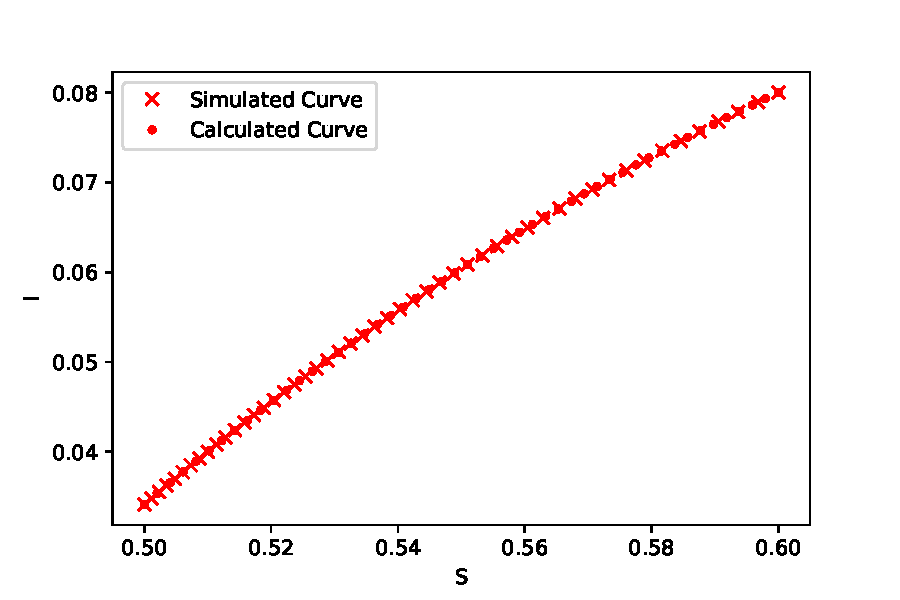
\includegraphics[width = \textwidth]{integral.pdf}
\caption{Curva simulada y calculada explícitamente. El tiempo de trayectoria obtenido para la curva se utilizó como punto final para la integración.}
\label{fig:integral}
\end{figure}

Se puede fijar un punto en $I$ y tomar una muestra de puntos en $S$ para generar diferentes trayectorias. De cada punto $s_0 \in S$, se puede obtener la trayectoria de menor tiempo y el punto $s_f$ en el que cruza \texttt{A.tau} (fig. \ref{fig:s0_vs_sf}). Estas mismas trayectorias se pueden graficar para ver cómo cambian las trayectorias <<óptimas>> con el punto inicial (fig. \ref{fig:short}).

\begin{figure}
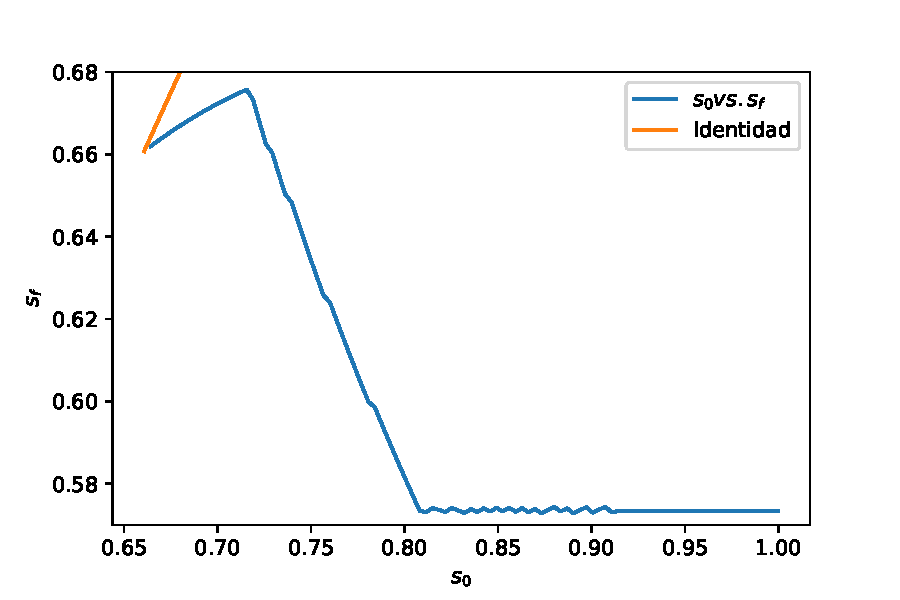
\includegraphics[width = \textwidth]{s0_vs_sf.pdf}
\caption{Punto inicial contra el punto final de la trayectoria de menor tiempo.}
\label{fig:s0_vs_sf}
\end{figure}

\begin{figure}
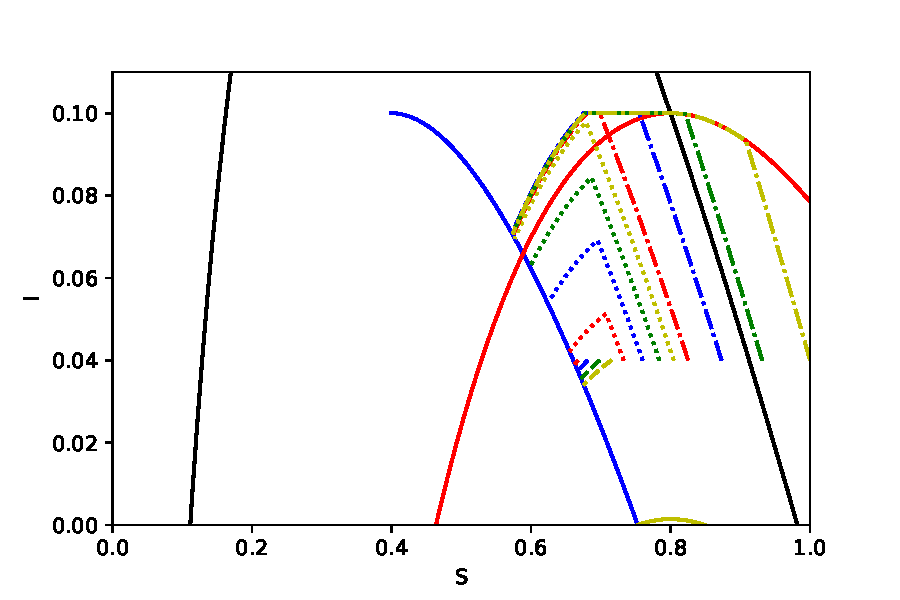
\includegraphics[width = \textwidth]{short_trajectories.pdf}
\caption{Se muestran diferentes trayectorias de las tres regiones de la figura \ref{fig:s0_vs_sf}. Las trayectorias con segmentos de línea ($--$) corresponden a la región de incremento. Las trayectorias con línea punteada ($\cdots$) a la región de decremento. Las trayectorias con líneas punteadas y segmento de línea ($-\cdot-$) corresponden a la región constante.}
\label{fig:short}
\end{figure}

\end{document}
